\documentclass{standalone}
% An example how to use the calendar library and modify the layout, i.e. put
% Sunday as the first week day.
%
% Author: Berteun Damman
\usepackage{tikz}
\usetikzlibrary{calendar}
\begin{document}
    \makeatletter
    \makeatother

    % The actual calendar is now rather easy:
    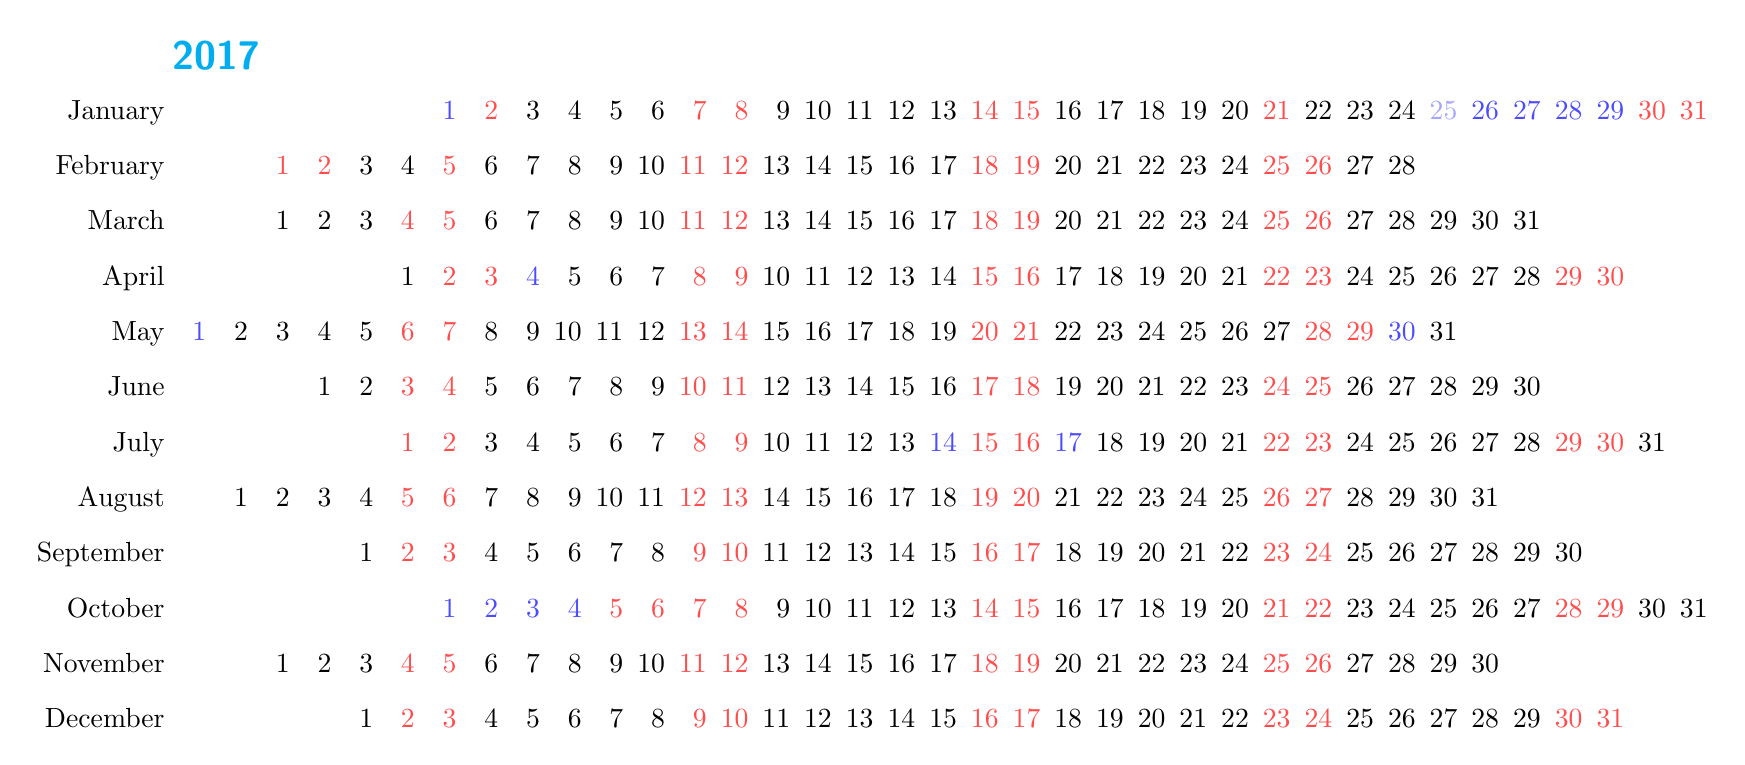
\begin{tikzpicture}
	\draw (0, 0) +(0,0.8) node [cyan, node font=\Large\sffamily\bfseries] {2017};
     \calendar[dates=2017-01-01 to 2017-12-last, month list, month label left, month yshift=2em]
        		if (weekend) [red!70]
        		if (equals=2017-01-01, between=2017-01-26 and 2017-01-29, equals=2017-04-04, equals=2017-05-01, equals=2017-05-30, equals=2017-07-14, equals=2017-07-17, between=2017-10-01 and 2017-10-04) [blue!70]
        		if (equals=2017-01-02, between=2017-01-30 and 2017-01-31, between=2017-02-01 and 2017-02-02, equals=2017-04-03, equals=2017-05-29, between=2017-10-05 and 2017-10-06) [red!70]
        		if (equals=2017-01-22, equals=2017-02-04, equals=2017-04-01, equals=2017-05-27, equals=2017-09-30) [black]
        		if (equals=2017-01-25) [blue!35]; 
    \end{tikzpicture}
\end{document}
